\usepackage{environ}

% Frame with a blue background, a blue title and a pink subtitle only.
\NewEnviron{frameD}[2]{
    \setbeamercolor{background canvas}{bg=afupbluebackground}

    \begin{frame}[noframenumbering]
        \begin{tikzpicture}[remember picture,overlay]
            \fill[afupblue] (0,0) rectangle(.05,\paperheight);
        \end{tikzpicture}
      \begin{tikzpicture}[remember picture,overlay]
          \ifx\insertframesubtitle\@empty%
              {\node[anchor=west, afupblue, font=\huge] at (0,.25){\uppercase\expandafter{#1}};}
          \else%
              {
                  \node[anchor= west, afupblue, font=\huge] at (0,.25){\uppercase\expandafter{#1}};%
                  \node[anchor= west, afuppink,font=\small] at (0,-.5){\uppercase\expandafter{#2}};}%
          \fi
      \end{tikzpicture}
    \end{frame}
  }

% Todo: Find a way to get rid of the top margin.
\NewEnviron{frameA}[2]{%
    \begin{frame}%
        \vspace{-.3cm}
        \begin{columns}[T]
            \column{\paperwidth}
            \begin{tikzpicture}
                \node[inner sep=0, outer sep=0, minimum height=.5\paperheight, minimum width=\textwidth] at (0,0){
                    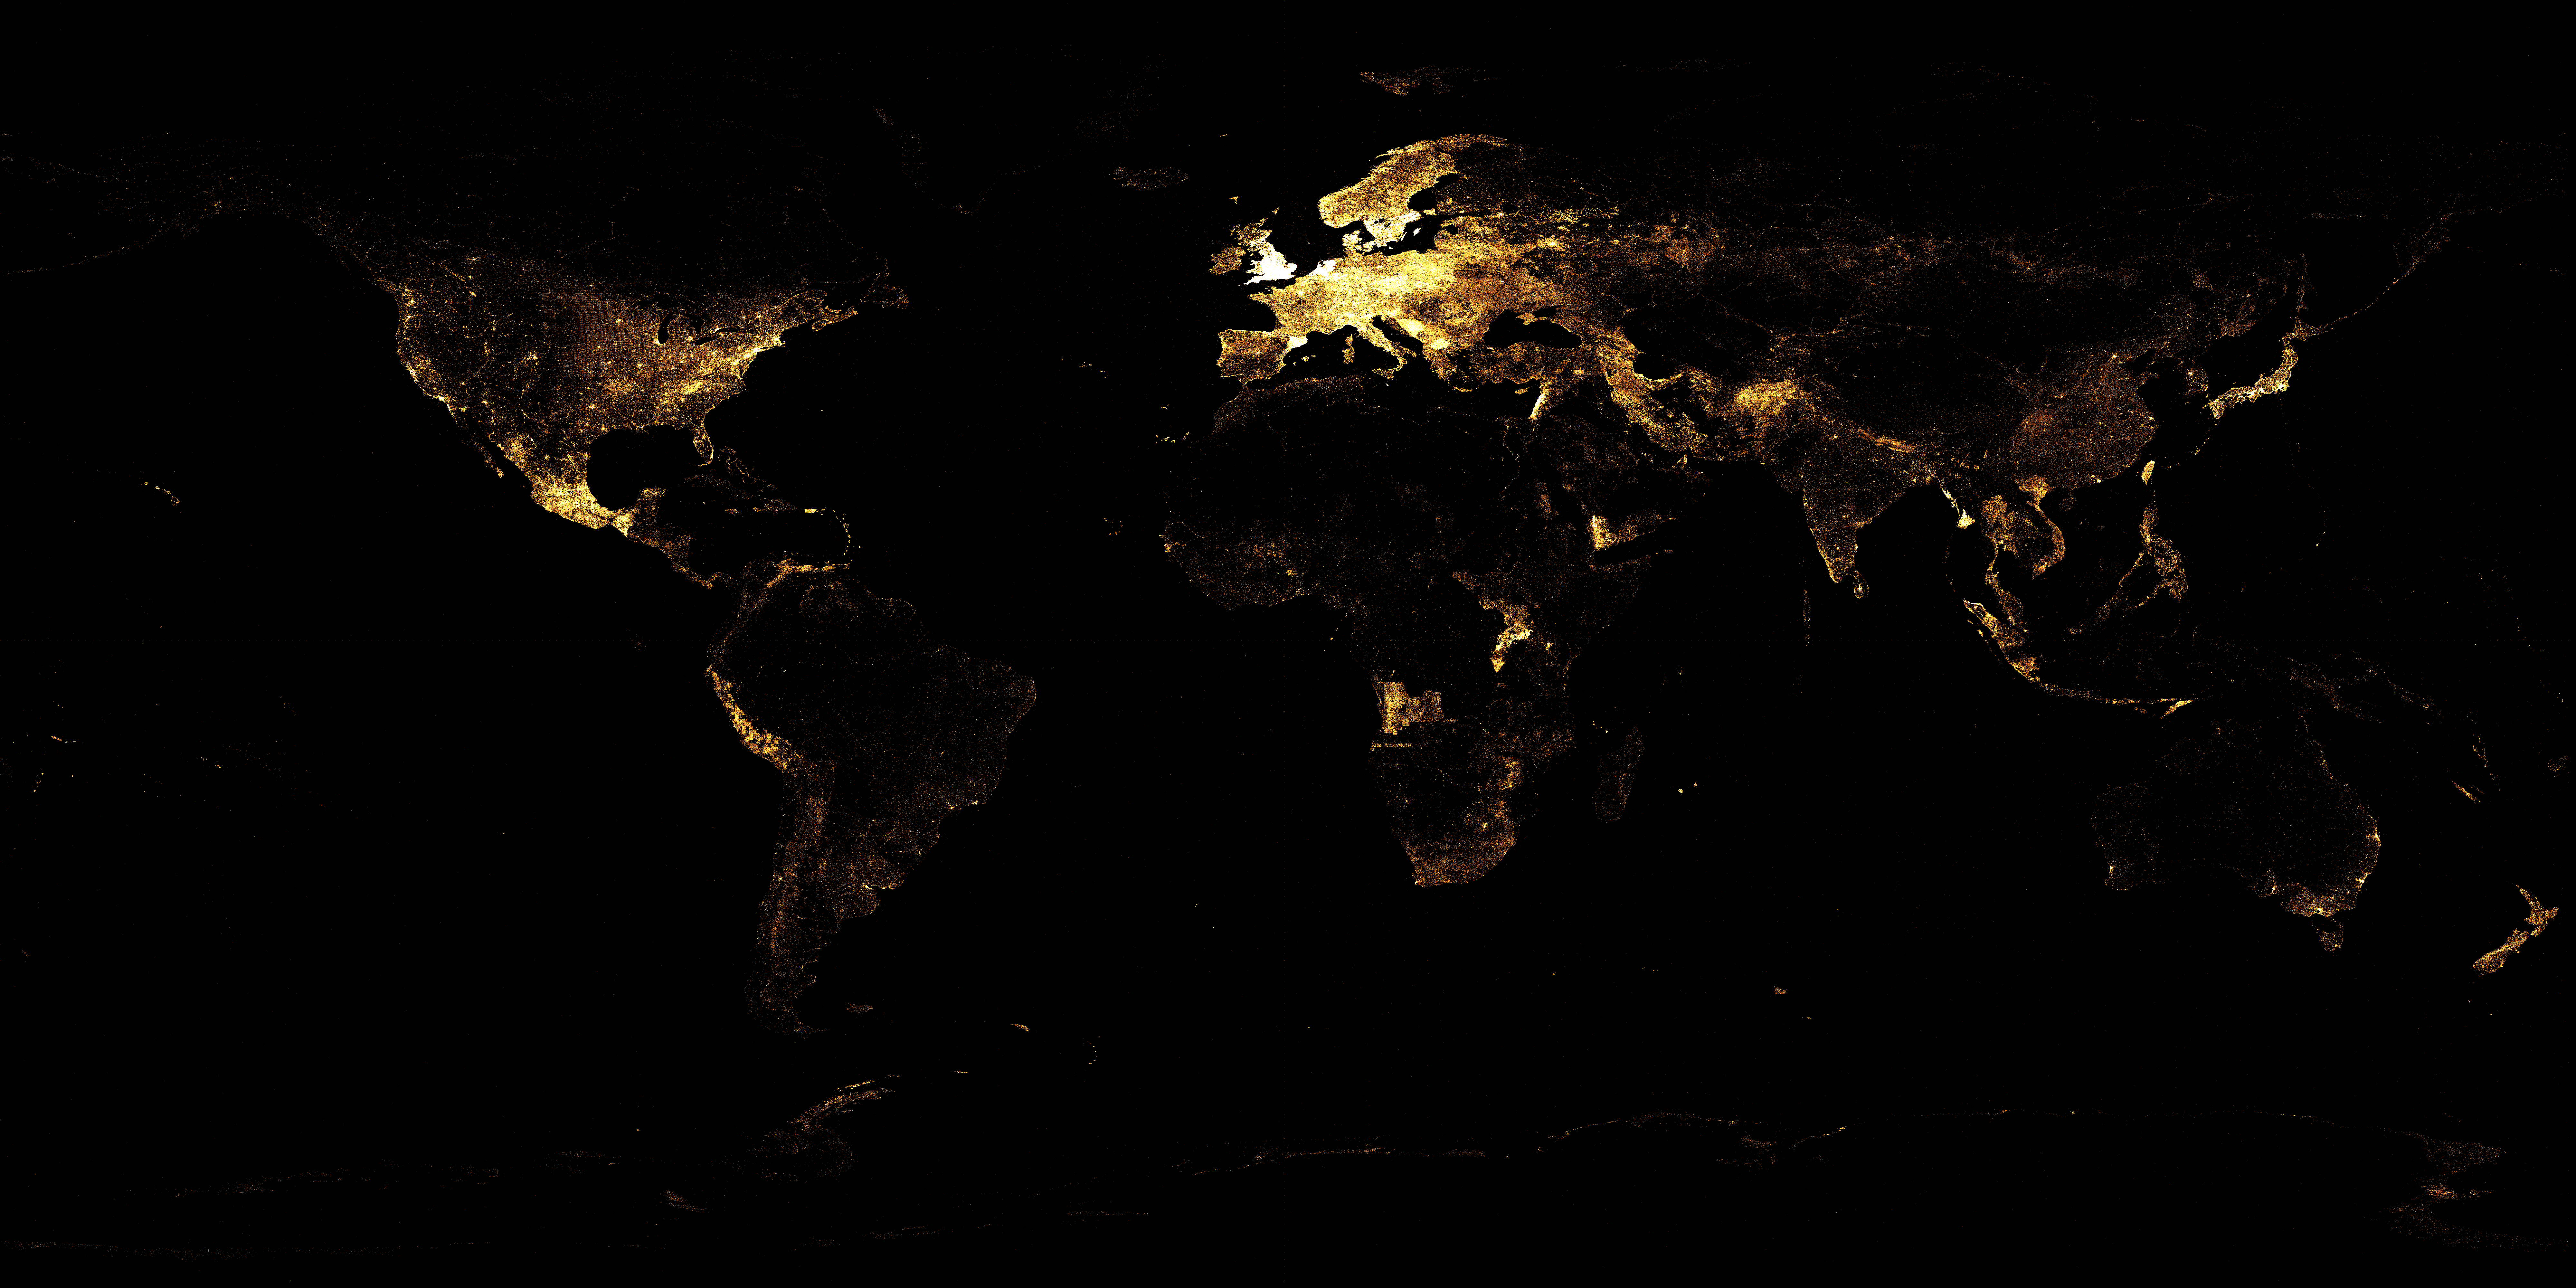
\includegraphics[width=\textwidth, height=.5\paperheight]{src/afup/style/logo/bg1}
                };
            \end{tikzpicture}
            \begin{tikzpicture}
                    \ifx\insertframesubtitle\@empty
                        {
                            \node[minimum height=.5\paperheight, minimum width=\textwidth, anchor=south] at (0,.25){\color{afupblue}\huge\uppercase\expandafter{#1}};
                        }
                    \else%
                        {
                            \node[minimum height=.5\paperheight, minimum width=\textwidth, anchor=south] at (0,.25){\color{afupblue}\huge\uppercase\expandafter{#1}};
                            \node[minimum height=.5\paperheight, minimum width=\textwidth, anchor=south] at (0,-.5){\color{afuppink}\small\uppercase\expandafter{#2}};
                        }%
                    \fi
                    \BODY%
            \end{tikzpicture}%
          \end{columns}%
    \end{frame}%
}

% Todo: Find a way to get rid of the top margin.
\NewEnviron{frameB}[2]{
    \begin{frame}
        \vspace{-.4cm}
        \begin{columns}[c]
            \column{.5\paperwidth}
                \begin{tikzpicture}
                    \node[inner sep=0, outer sep=0, minimum height=\paperheight, minimum width=\textwidth] at (0,0){
                        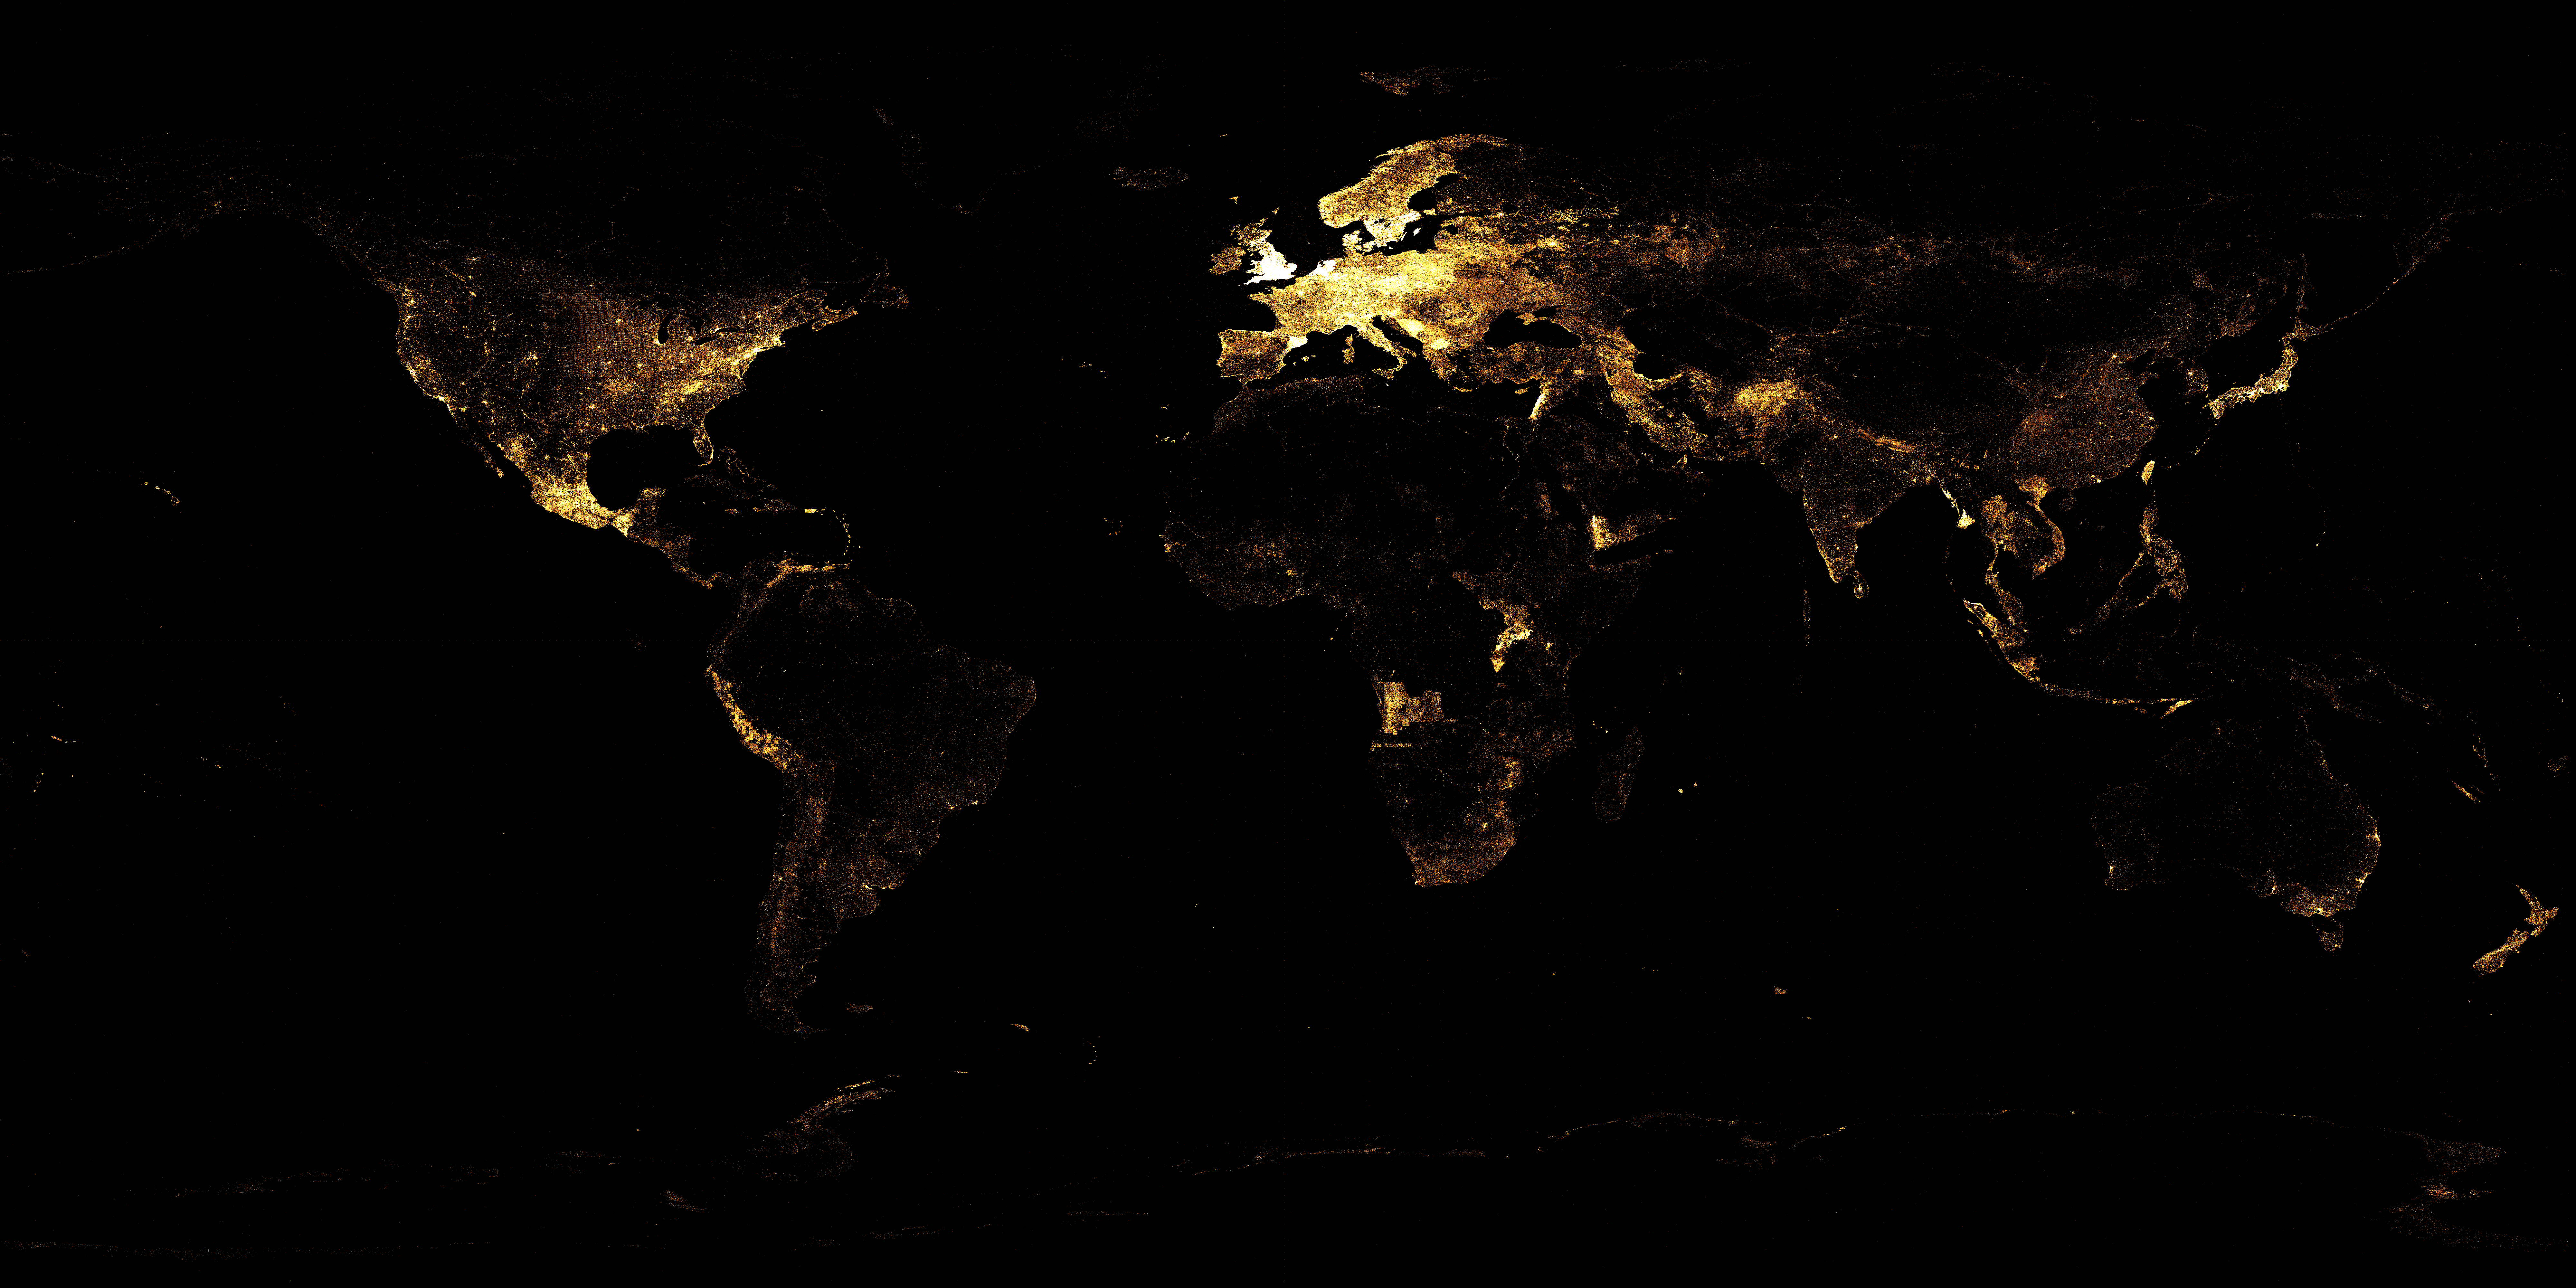
\includegraphics[width=\textwidth, height=\paperheight]{src/afup/style/logo/bg1}
                    };
                \end{tikzpicture}
            \column{.5\paperwidth}
                \begin{tikzpicture}
                    \ifx\insertframesubtitle\@empty
                        {
                            \node[shape=rectangle, text opacity=1,minimum height=\paperheight, minimum width=\textwidth, anchor=south, afupblue, font=\huge] at (0,.25){\uppercase\expandafter{#1}};
                        }
                    \else
                        {
                            \node[shape=rectangle, text opacity=1,minimum height=\paperheight, minimum width=\textwidth, anchor=south, afupblue, font=\huge] at (0,.25){\uppercase\expandafter{#1}};
                            \node[shape=rectangle, text opacity=1,minimum height=\paperheight, minimum width=\textwidth, anchor=south, afuppink, font=\small] at (0,-.5){\uppercase\expandafter{#2}};
                        }
                    \fi
                    \BODY
                \end{tikzpicture}
        \end{columns}
    \end{frame}
}

\NewEnviron{frameC}[2]{%
    \setbeamercolor{background canvas}{bg=white}

    \begin{frame}[noframenumbering]
        \begin{center}
            \ifx\insertframesubtitle\@empty%
                {
                    \color{afupblue}
                    \huge\uppercase\expandafter{#1}
                }
            \else%
                {
                    \color{afupblue}
                    \huge\uppercase\expandafter{#1}
                    \noindent
                    {\color{afuppink} \rule{\linewidth}{0.5mm}}
                    \color{afuppink}
                    \small\uppercase\expandafter{#2}
                }%
            \fi
    \end{center}
\end{frame}
}

% To read: https://tex.stackexchange.com/questions/113410/removing-sidebar-from-a-single-beamer-frame
% To read: https://github.com/deuslirio/UFGTeX-Presentation
% To read: https://github.com/matze/mtheme
